\pagebreak
\section{Figures}

% Figures for Gaussian process
\begin{figure}[H]
  \centering
  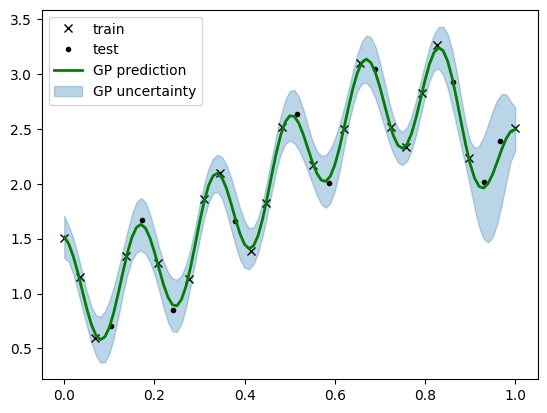
\includegraphics[width=.65\textwidth]{./figures/map_pred.png}
  \caption{
    Prediction using MAP.
  }
  \label{fig:gp:map:pred}
\end{figure}
%
\begin{figure}[H]
  \centering
  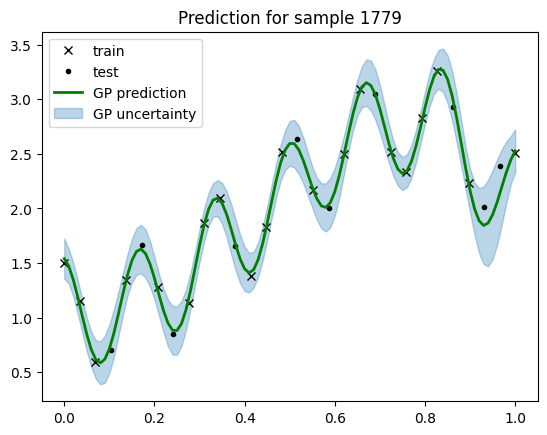
\includegraphics[width=.65\textwidth]{./figures/nuts_pred.png}
  \caption{
    Random prediction using NUTS.
  }
  \label{fig:gp:nuts:pred}
\end{figure}

\begin{figure}[p]
  \centering
  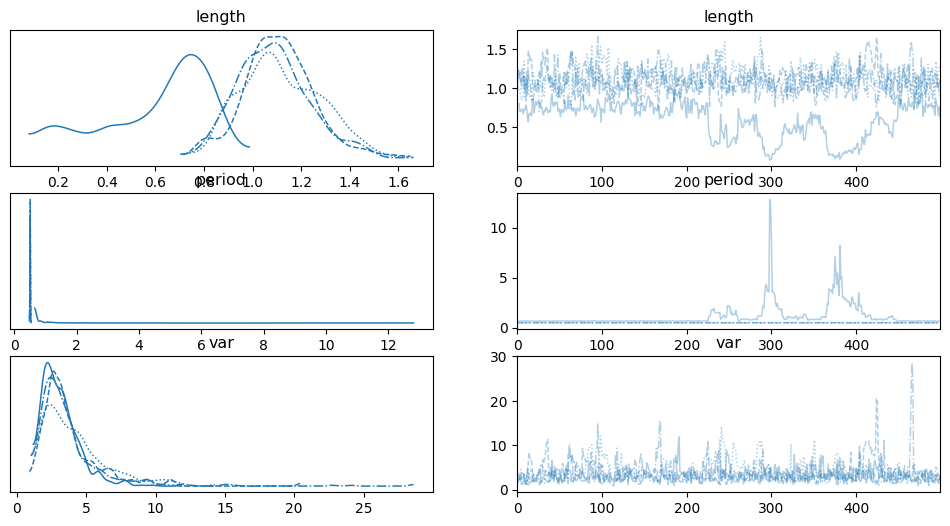
\includegraphics[width=1\textwidth]{./figures/nuts_trace.png}
  \caption{
    Sample trace for the 4 different chains over model parameters.
  }
  \label{fig:gp:nuts:trace}
\end{figure}
%
\begin{figure}[p]
  \centering
  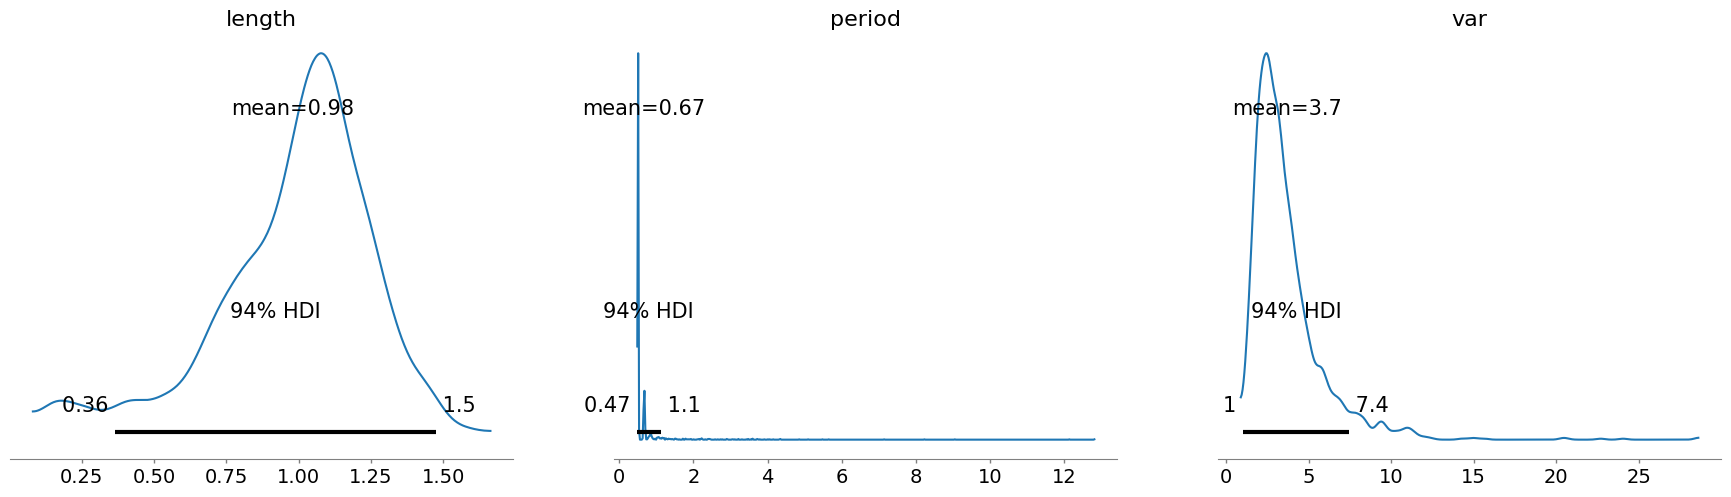
\includegraphics[width=1\textwidth]{./figures/nuts_post.png}
  \caption{
    Posterior samples of the parameters of the model.
  }
  \label{fig:gp:nuts:post}
\end{figure}

\begin{figure}[p]
  \centering
  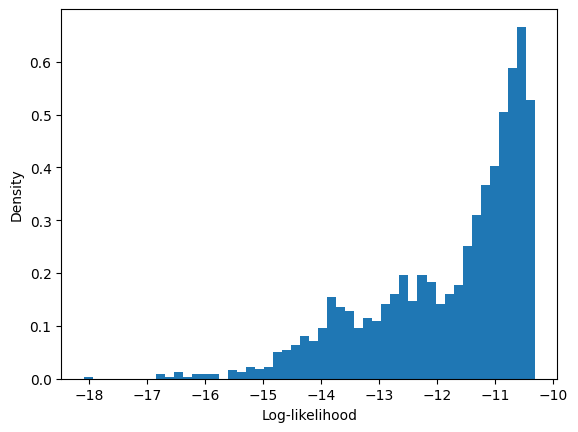
\includegraphics[width=.8\textwidth]{./figures/nuts_ll.png}
  \caption{
    Distribution of log-likelihoods of test data
    from posterior samples using NUTS.
  }
  \label{fig:gp:nuts:ll}
\end{figure}
%
\begin{figure}[p]
  \centering
  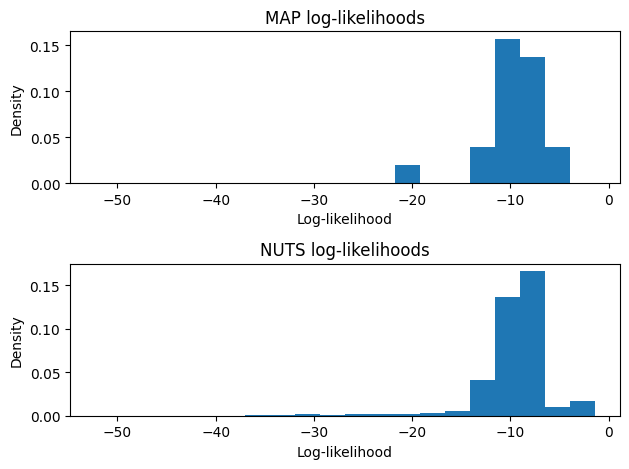
\includegraphics[width=0.6\textwidth]{./figures/map_nuts_ll.png}
  \caption{
    Comparing log-likelihoods when using MAP and NUTS.
  }
  \label{fig:gp:map_nuts_ll}
\end{figure}

\begin{figure}[p]
  \centering
  \begin{subcaptionblock}{.5\textwidth}
    \centering
    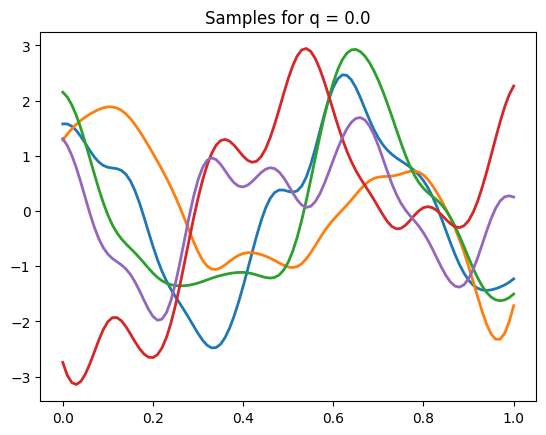
\includegraphics[width=\textwidth]{./figures/gp_constr_q0.png}
  \end{subcaptionblock}
  \\
  \begin{subcaptionblock}{.5\textwidth}
    \centering
    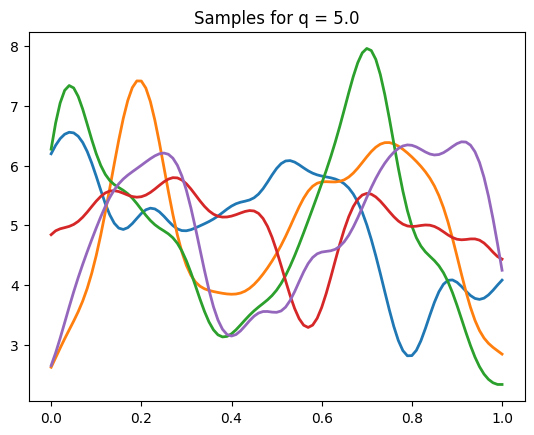
\includegraphics[width=\textwidth]{./figures/gp_constr_q5.png}
  \end{subcaptionblock}
  \\
  \begin{subcaptionblock}{.5\textwidth}
    \centering
    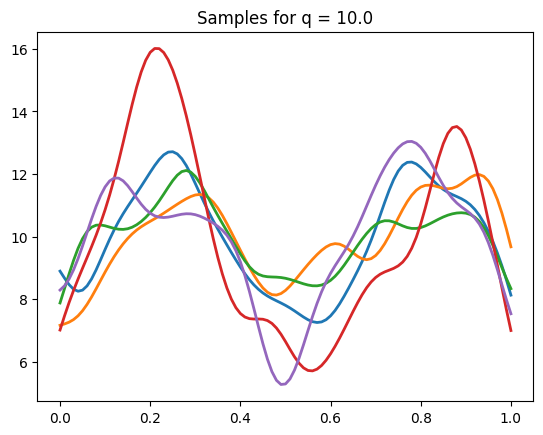
\includegraphics[width=\textwidth]{./figures/gp_constr_q10.png}
  \end{subcaptionblock}
  \caption{Samples from $f | X, \hat{q}$ for $q \in \{ 0, 5, 10 \}$.}
  \label{fig:gp:constrained:samples}
\end{figure}

\begin{figure}[p]
  \centering
  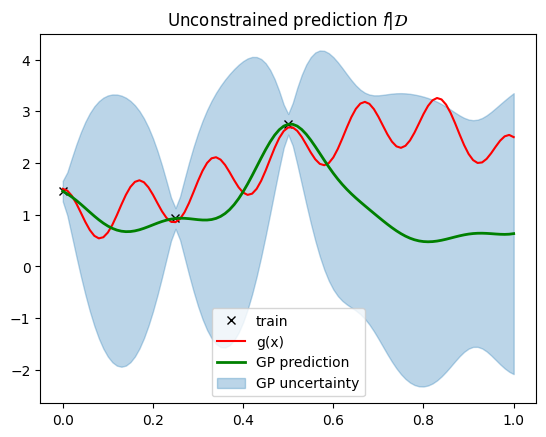
\includegraphics[width=0.65\textwidth]{./figures/gp_pred_unconstrained.png}
  \caption{
    Plot of unconstrained posterior $f | \mathcal{D}$.
  }
  \label{fig:gp:pred:unconstrained}
\end{figure}
